% !TeX root = ../../../main.tex
\section{Architektura sieci Mask R-CNN}
\label{sec:architekrura_mask_rcnn}

\textit{Mask R-CNN} \cite{matterport-mask-rcnn} (z ang. \textit{Mask Regions with Convolutional Neural Network}) jest implementacją o otwartym kodzie źródłowym modelu do segmentacji instancji opisanego w publikacji o tej samej nazwie, \textit{Mask R-CNN} \cite{general-mask-rcnn}.
W celu zrozumienia tego modelu, najlepiej rozważać go w kontekście ewoluowania kolejnych iteracji, którego końcowym rezultatem jest \textit{Mask R-CNN}.

\subsection{Iteracja pierwsza - R-CNN}

\TODO{Tu będzie schemat R-CNN}
\TODO{Tu będzie wyjaśnienie schematu}

\textit{R-CNN} \cite{rcnn} (z ang. \textit{Regions with Convolutional Neural Network}), przedstawiony w 2014 roku, rozwiązuje zagadnienie detekcji obiektów na obrazie (to znaczy wskazuje konkretne obiekty, ale bez konkretnych pikseli).
Działanie modelu można zobrazować w następujących krokach:

\begin{enumerate}
  \item najpierw na obszarze obrazu wejściowego generowane są tzw. propozycje regionów, przy użyciu algorytmu \textit{Selective Search} \cite{selective-search}; celem jest znalezienie regionów, w których prawdopodobnie znajduje się jakiś obiekt;
	\item następnie, dla każdego takiego regionu wydobywane są cechy za pomocą \textit{CNN};
  \item w dalszej kolejności, cechy każdego regionu analizowane są przez model wektorów nośnych; wynikiem jest klasyfikacja regionu na dwie grupy - wskazany obiekt lub brak obiektu;
	\item na końcu dla regionów, w których wskazano obiekt następuje próba dopasowania obszaru do rozmiaru obiektu - wynikiem jest obwódka (z ang. \textit{bounding box}) wskazująca położenie obiektu na obrazie.
\end{enumerate}

\newpage
\subsection{Iteracja druga - Fast R-CNN}

\TODO{Tu będzie schemat Fast R-CNN}
\TODO{Tu będzie wyjaśnienie schematu}

\textit{Fast R-CNN} \cite{fast-rcnn}, przedstawiony w 2015 roku, usprawnia model \textit{R-CNN}, w którym zidentyfikowano następujące problemy:

\begin{itemize}
  \item problem w implementacji i w wytrenowaniu sieci wynikający z samej budowy \textit{R-CNN}; \textit{R-CNN} składa się z~czterech części, które osobno wymagają zrozumienia, implementacji i trenowania lub doboru parametrów:
		\begin{itemize}
			\item \textit{Selective Search} do generowania regionów;
			\item \textit{CNN} do ekstrakcji cech;
			\item \textit{SVM} do klasyfikacji;
			\item model dopasowujący obwódkę.
		\end{itemize}
  \item zduplikowane obliczenia na etapie ekstrakcji cech, wynikające z faktu, że ekstracja cech uruchamiana jest dla każdego regionu, a gdy regiony zachodzą na siebie, obliczenia ekstrakcji cech są powtarzane.
\end{itemize}

Używając \textit{Fast R-CNN} ekstrakcja cech następuje następuje tylko raz, na początku.
W ten sposób powstaje mapa cech całego obrazu.
Gdy zachodzi konieczność ekstrakcji cech regionu, zamiast liczyć cechy od nowa, wyciągany jest odpowiadający fragment mapy cech.
Metoda ta to tzw. \textit{Region of Interest Pooling} \cite{region-of-interest-pooling}.

Oprócz zmian w sposobie liczenia cech, w \textit{Fast R-CNN} klasyfikator \textit{SVM} został zastąpiony siecią neuronową.
Podobnie stało się z~modelem dopasowującym obwódkę.
Te dwie nowe sieci połączono w jedną sieć wraz z~siecią \textit{CNN}.
Podsieć klasyfikująca i podsieć dopasowująca obwódke zostały włączone do sieci w sposób równoległy, to znaczy ich wyniki nie zależą od siebie nawzajem.

Zmiany te rozwiązały w dużej części problemy \textit{R-CNN} wymienione powyżej.

\newpage
\subsection{Iteracja trzecia - Faster R-CNN}

\TODO{Tu będzie schemat Faster R-CNN}
\TODO{Tu będzie wyjaśnienie schematu}

\textit{Faster R-CNN} \cite{faster-rcnn}, przedstawiony w 2016 roku, wprowadza kolejne usprawnienie, którego zabrakło w \textit{Fast R-CNN}.
Chodzi o generowanie regionów za pomocą algorytm \textit{Selective Search} \cite{selective-search}, który działał stosunkowo wolno.
Usprawnienie polegało na zastąpieniu algorytmu nową siecią neuronową, która korzysta z~cech obrazu do generowania regionów.
Jako że sieć została włączona do modelu w taki sposób, że bazuje na wyznaczonej mapie cech, to uzyskano w ten sposób znacznie szybszy model.
Dodatkowo był to kolejny krok zastępujący część modelu podsiecią neuronową, w wyniku czego model stał się jedną siecią neuronową składającą się z~podsieci:

\begin{itemize}
	\item budującej mapę cech;
	\item generującej regiony;
	\item klasyfikującej;
	\item dopasowującej obwódkę.
\end{itemize}

\subsection{Iteracja czwarta - Mask R-CNN}

Schemat \textit{Mask R-CNN} przedstawiony jest na rysunku \myfigref{fig:mask_r_cnn}.

\TODO{Tu będzie wyjaśnienie schematu}

\textit{Mask R-CNN}, przedstawiony w 2017 roku, stanowi ostatni krok w opisanej ewolucji modelu.
Do dwóch równoległych podsieci - klasyfikującej oraz zacieśniającej obwódkę - wprowadza nową, równoległą podsieć odpowiedzialną za wskazywanie konkretnych pikseli wykrytego obiektu.

\begin{figure}[h]
  \centering
  \caption{Schemat sieci Mask R-CNN}
  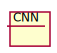
\includegraphics[width=1\textwidth]{mask_r-cnn.png}
  \label{fig:mask_r_cnn}
\end{figure}
